
\begin{frame}
    \frametitle{Description}
    \begin{itemize}
        \item Here, the back propagation algorithm has been implemented for
            a single hidden layer network.
        \item This network was made for fun as a part of the course work called
            ``Foundations of machine learning".
        \item Both the hidden layer and output layer have sigmoid as activation
            function
        \item The code was tested on the following problems
            \begin{itemize}
                \item XOR Gate problem
                \item $y=f(x)$ function approximation problem
            \end{itemize}
        \item The class notes on this is attached at the end of this presentation.
    \end{itemize}
\end{frame}

%------------------------------------------------------------------------------
\begin{frame}
    \centering
    \usebeamercolor[fg]{title}\usebeamerfont{title} Problem 1 \\ \vspace{1cm} XOR Gate problem
\end{frame}

\begin{frame}
    \frametitle{XOR Gate problem}
    Aim is to approximate the XOR gate with a single hidden layer network.
    \begin{table}
        \caption{XOR Gate truth table}
        \begin{tabular}{ccc}
        \toprule
            \(X_1\) & \(X_2\) & \(Y\) \\ \midrule
            0 & 0 & 0 \\
            1 & 0 & 1 \\
            0 & 1 & 1 \\
            1 & 1 & 0 \\ \bottomrule
        \end{tabular}
    \end{table}
\end{frame}

\begin{frame}
    \frametitle{XOR Gate problem - network schematic}
    Network with two inputs, two neurons in hidden layer and one output
    \vspace{1cm}
    \begin{figure}
        \center
        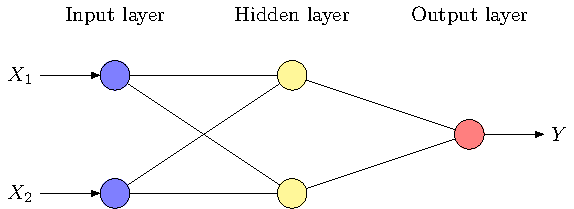
\includegraphics[scale=1]{supportingFiles/schematics/XOR_problem/XOR_schematic.pdf}
        \caption{Network schematic}
    \end{figure}
\end{frame}

\begin{frame}
    \frametitle{XOR Gate problem - Loss graph}
    \begin{figure}
        \center
        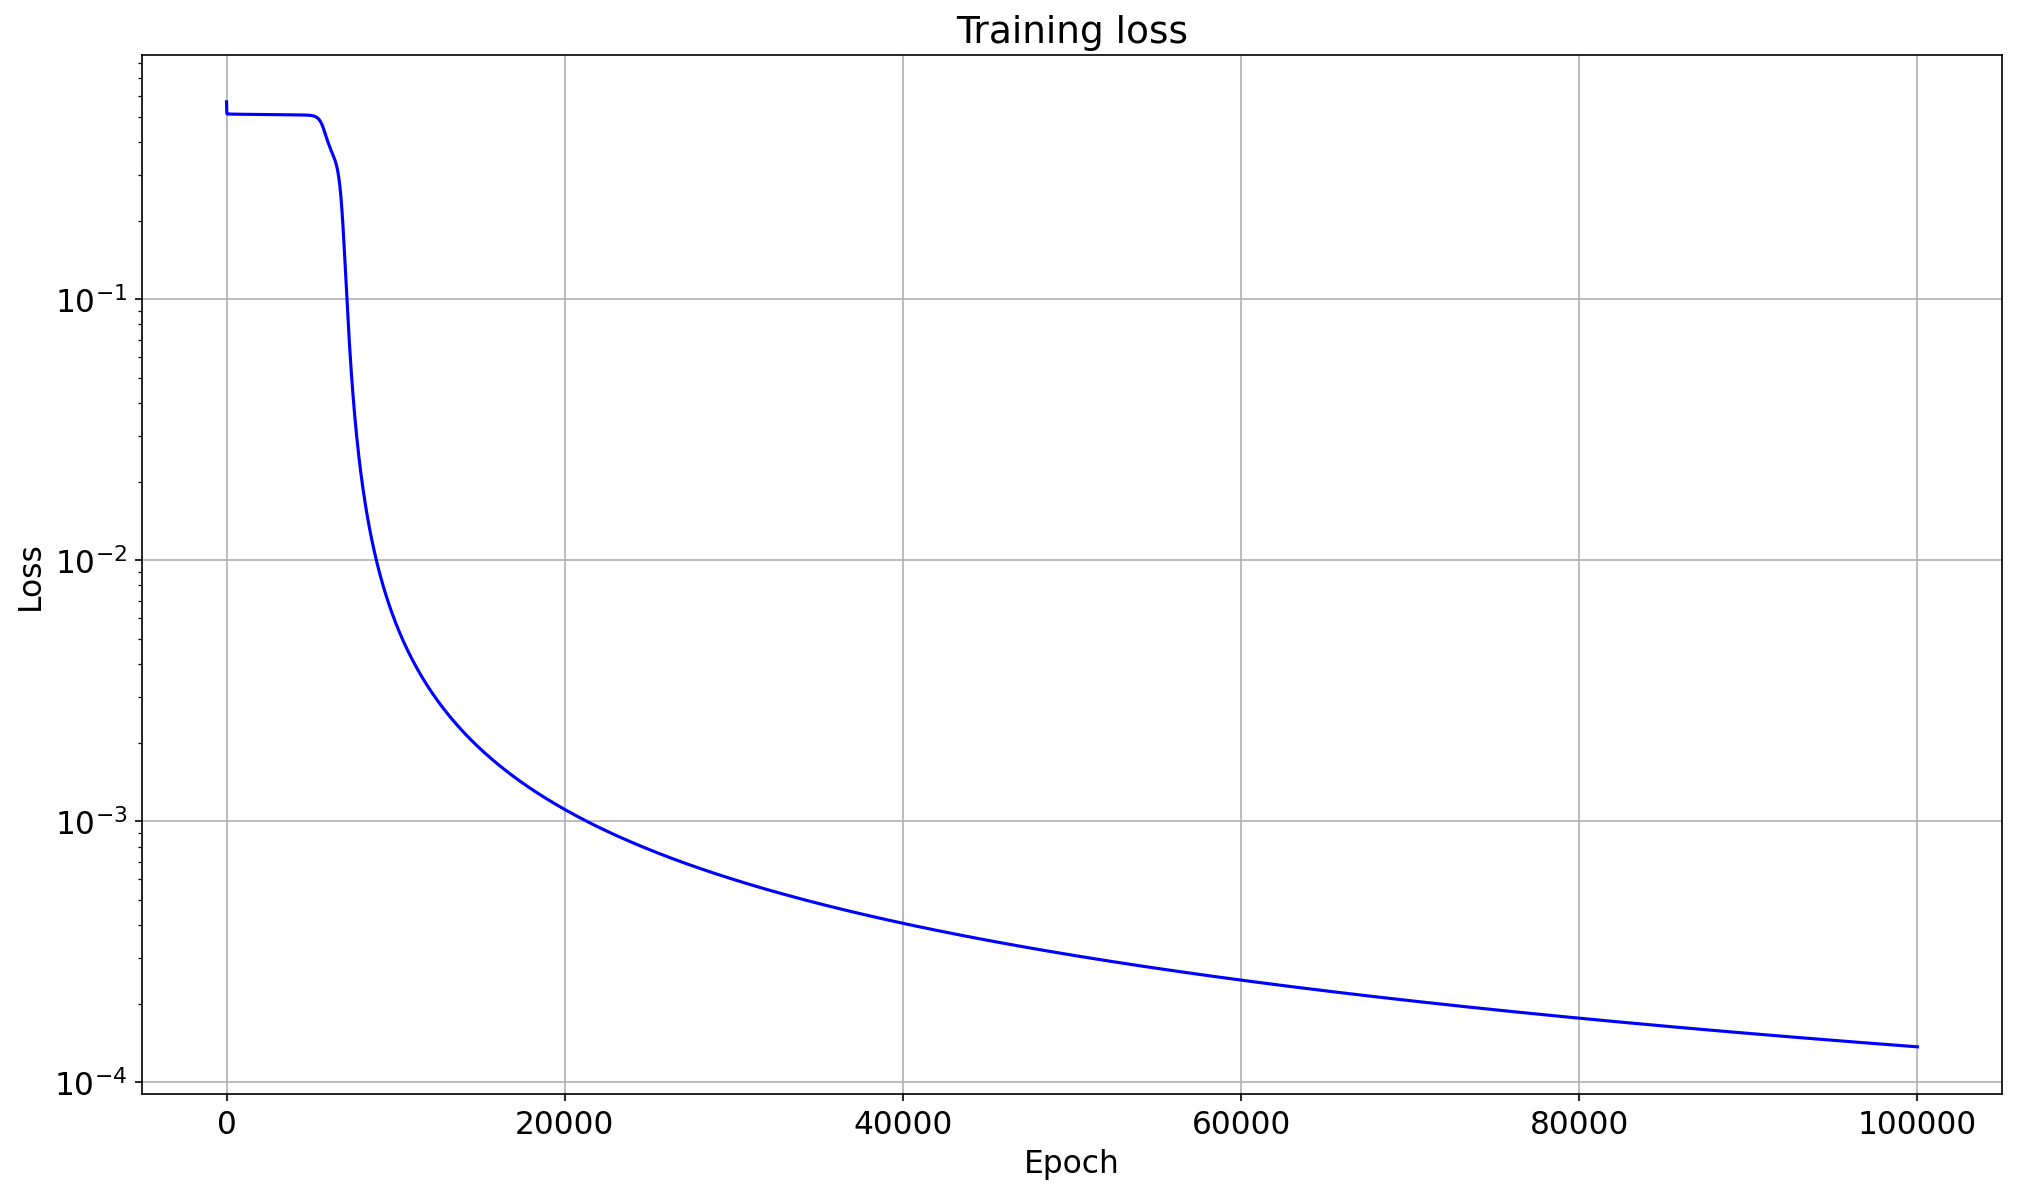
\includegraphics[scale=0.33]{supportingFiles/lossGraphs/loss_XOR.png}
        \caption{Training loss profile for XOR problem}
    \end{figure}
\end{frame}

\begin{frame}
    \frametitle{XOR Gate problem - Estimation}
    \begin{table}
        \caption{Network estimated values $\hat{Y}$ compared with XOR Truth Table}
        \begin{tabular}{cccc}
        \toprule
            $X_1$ & $X_2$ & $Y$ & $\hat{Y}$ \\ \midrule
            0 & 0 & 0 & 0.0075 \\
            1 & 0 & 1 & 0.9921 \\
            0 & 1 & 1 & 0.9921 \\
            1 & 1 & 0 & 0.0096 \\ \bottomrule
        \end{tabular}
    \end{table}
\end{frame}

%------------------------------------------------------------------------------
\begin{frame}
    \centering
    \usebeamercolor[fg]{title}\usebeamerfont{title} Problem 2 \\ \vspace{1cm}  Function \(y = f(x)\) approximation
\end{frame}

\begin{frame}
    \frametitle{$y=f(x)$ function approximation}
    Aim is to make the network to approximate a simple $y = f(x)$ function profile.
    \vspace{0.25cm}
    \begin{figure}
        \center
        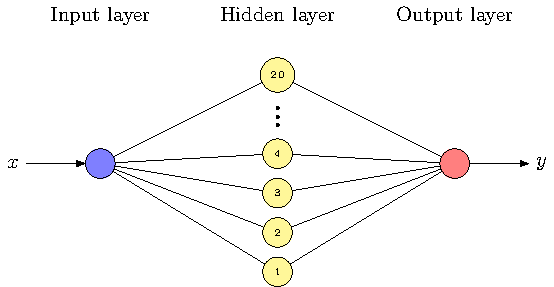
\includegraphics[scale=1]{supportingFiles/schematics/XY_problem/XY_schematic.pdf}
        \caption{Network schematic, with 20 neurons in the hidden layer}
    \end{figure}
\end{frame}

\begin{frame}
    \frametitle{$y=f(x)$ function approximation - Loss graph}
    \begin{figure}
        \center
        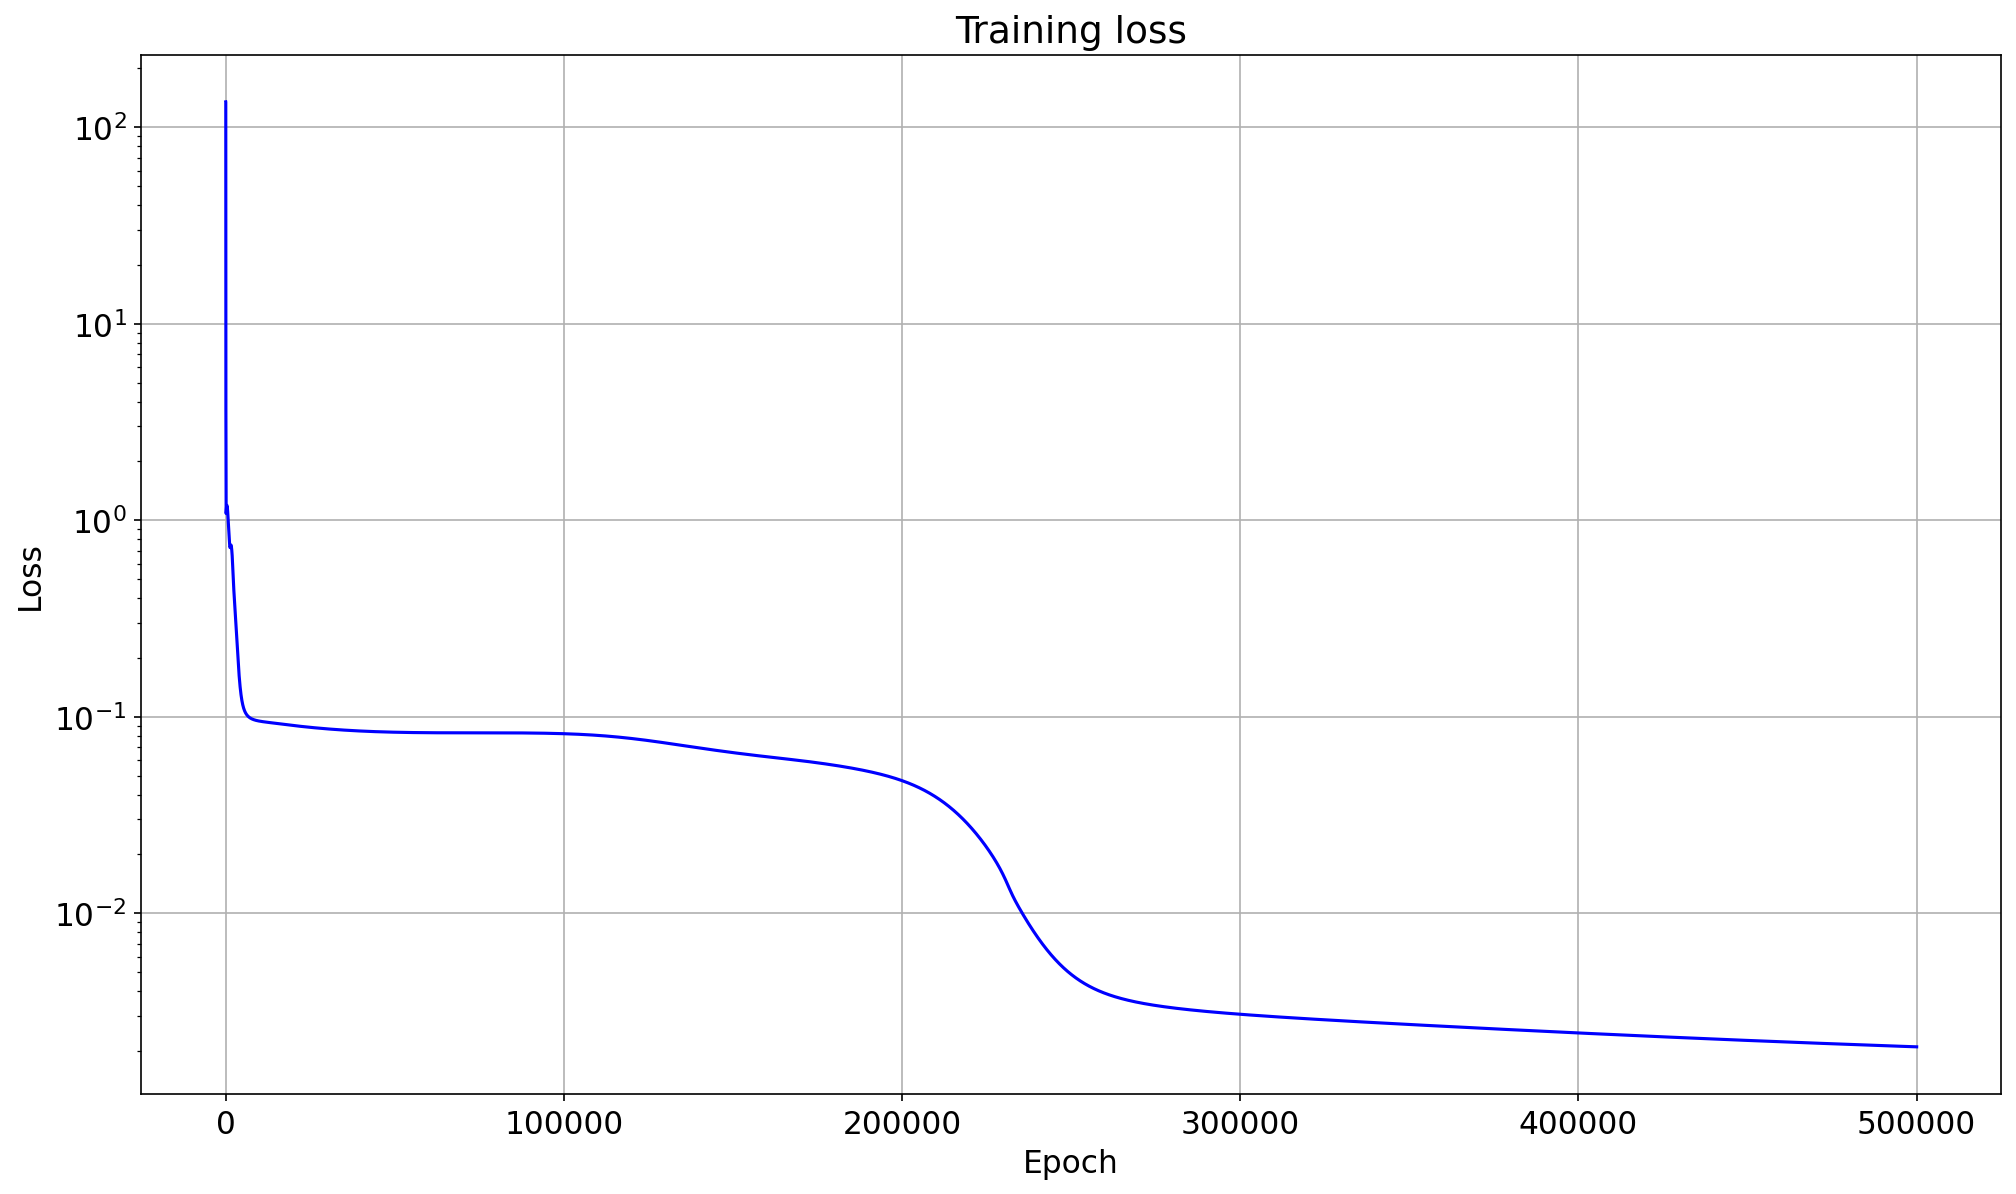
\includegraphics[scale=0.33]{supportingFiles/lossGraphs/loss_XY.png}
        \caption{Training loss profile for the function $y=f(x)$ approximation}
    \end{figure}
\end{frame}

\begin{frame}
    \frametitle{$y=f(x)$ function approximation - Estimation}
    \begin{figure}
        \center
        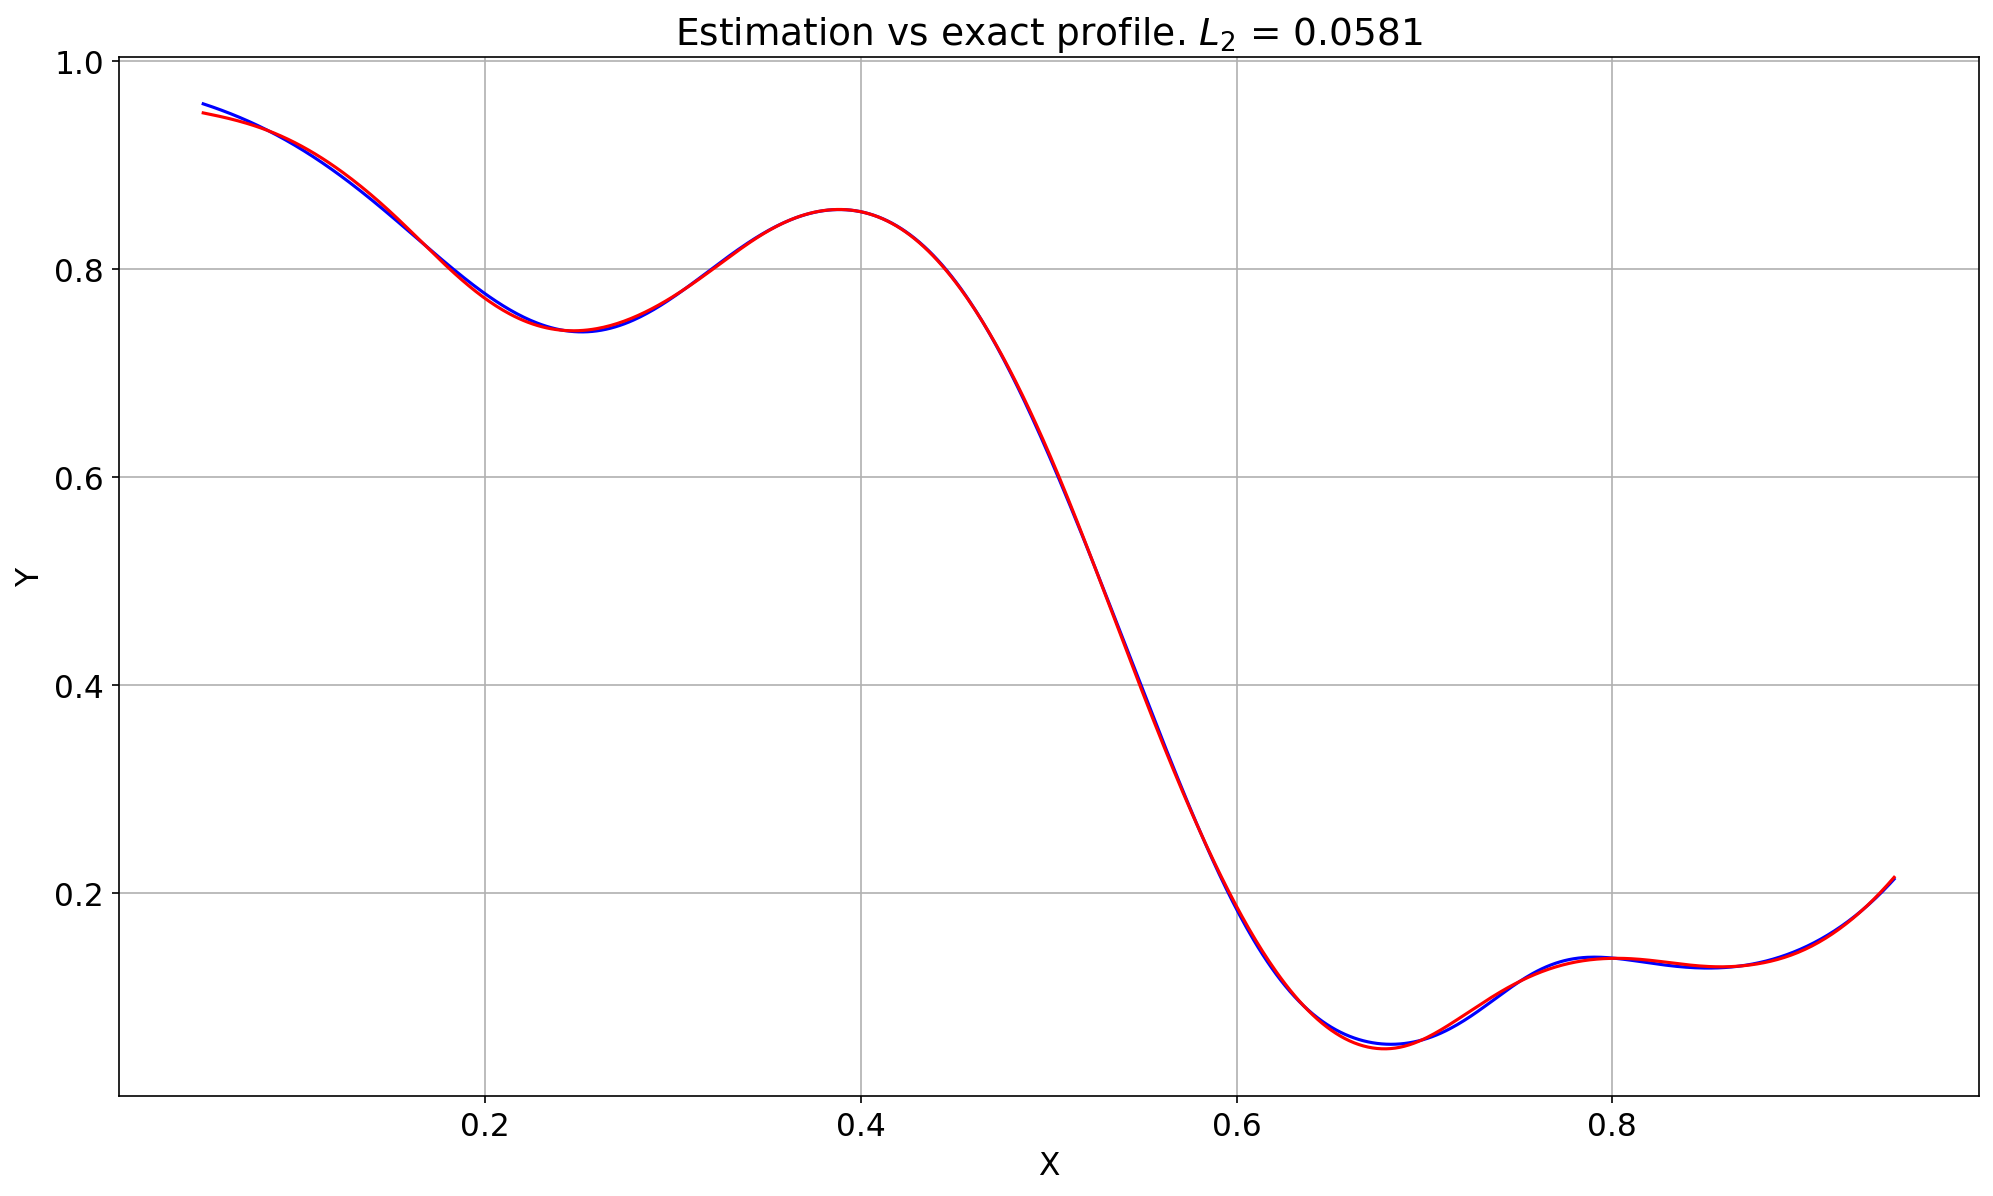
\includegraphics[scale=0.33]{supportingFiles/results/prediction_XY.png}
        \caption{Estimated vs exact output of the function $y=f(x)$}
    \end{figure}
\end{frame}

%------------------------------------------------------------------------------
\begin{frame}
   \centering
    \usebeamercolor[fg]{title}\usebeamerfont{title} Following are the class notes regarding back propagation algorithm
\end{frame}

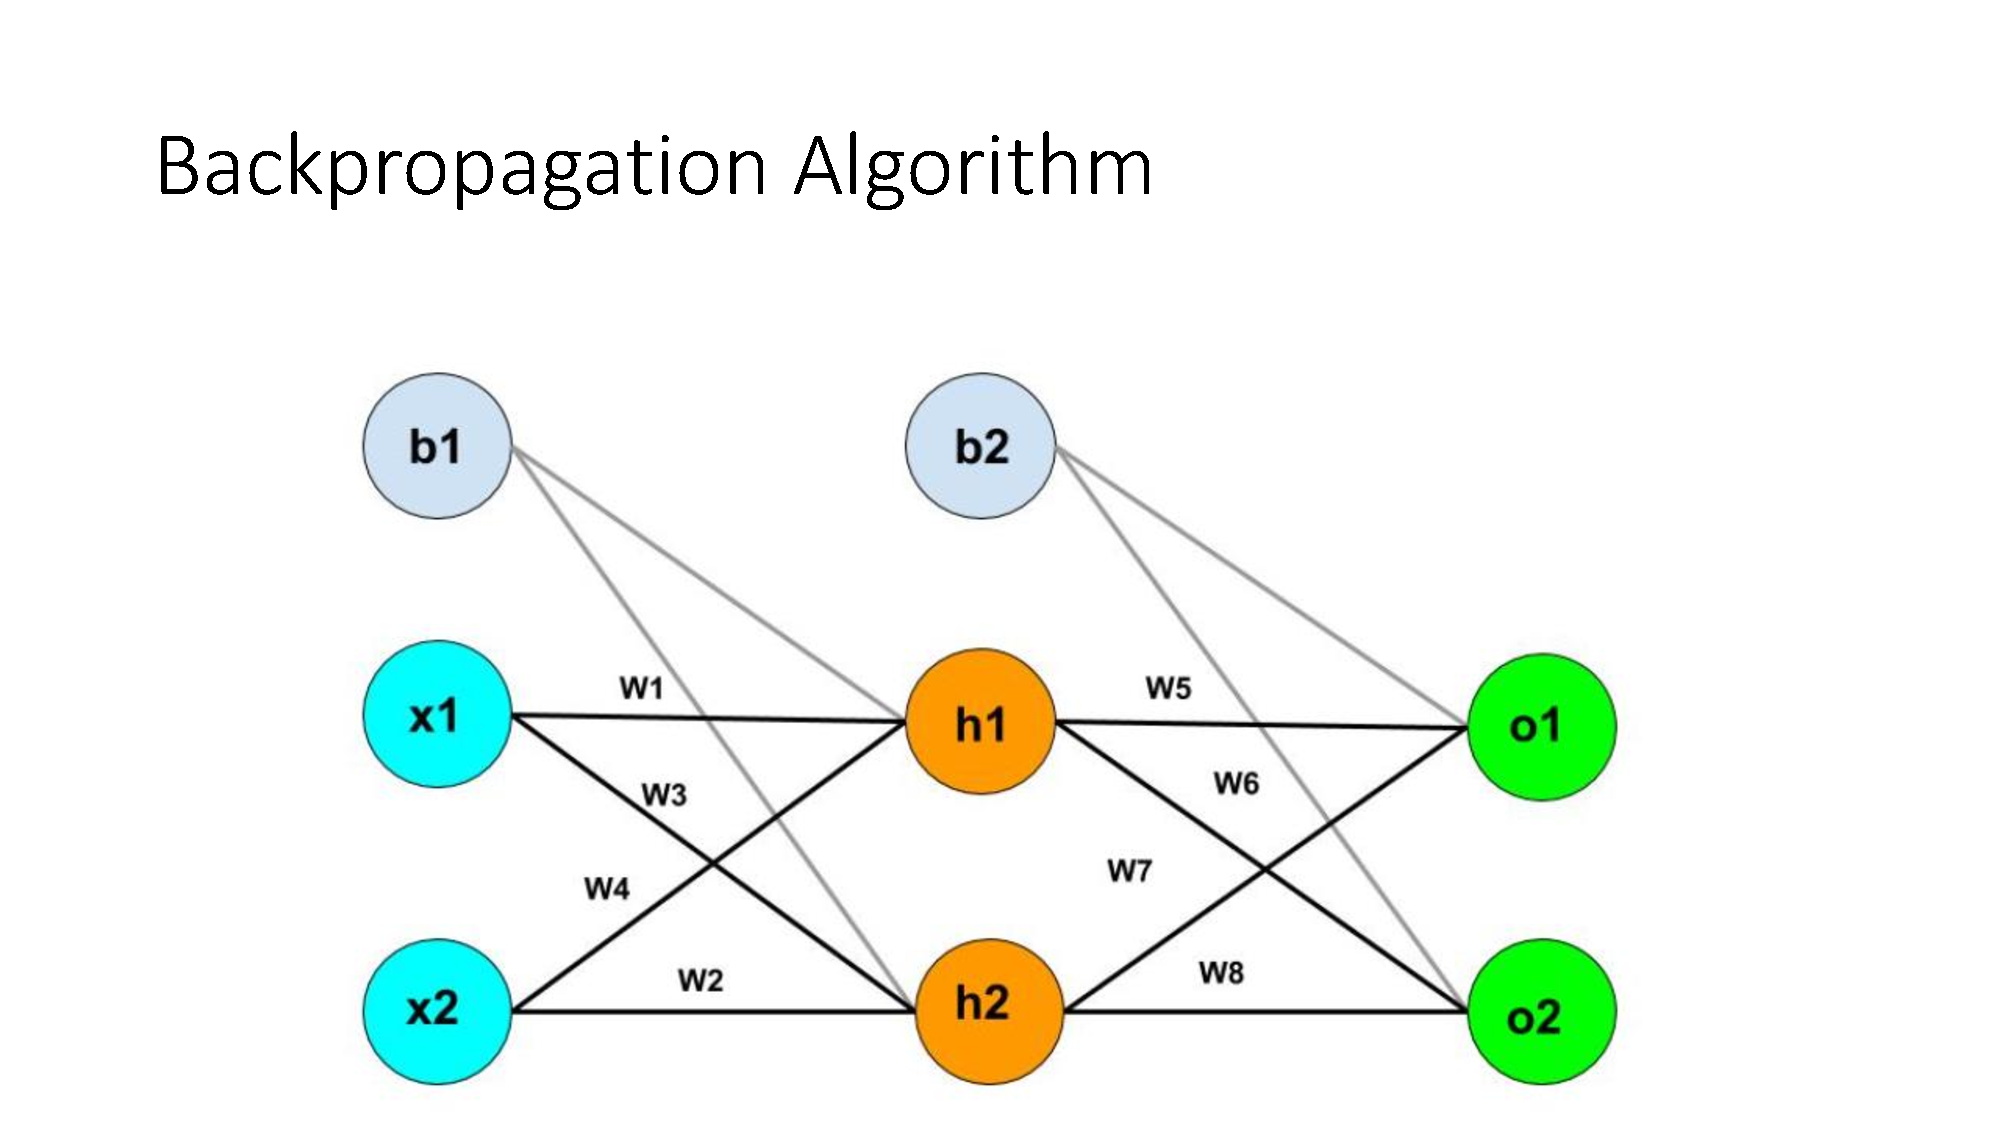
\includepdf[pages={-}]{supportingFiles/classNotes/Backpropagation_Algorithm.pdf}


\begin{frame}
   \centering
    \usebeamercolor[fg]{title}\usebeamerfont{title} Thank you!
\end{frame}
